% Options for packages loaded elsewhere
\PassOptionsToPackage{unicode}{hyperref}
\PassOptionsToPackage{hyphens}{url}
%
\documentclass[
]{article}
\usepackage{lmodern}
\usepackage{amssymb,amsmath}
\usepackage{ifxetex,ifluatex}
\ifnum 0\ifxetex 1\fi\ifluatex 1\fi=0 % if pdftex
  \usepackage[T1]{fontenc}
  \usepackage[utf8]{inputenc}
  \usepackage{textcomp} % provide euro and other symbols
\else % if luatex or xetex
  \usepackage{unicode-math}
  \defaultfontfeatures{Scale=MatchLowercase}
  \defaultfontfeatures[\rmfamily]{Ligatures=TeX,Scale=1}
\fi
% Use upquote if available, for straight quotes in verbatim environments
\IfFileExists{upquote.sty}{\usepackage{upquote}}{}
\IfFileExists{microtype.sty}{% use microtype if available
  \usepackage[]{microtype}
  \UseMicrotypeSet[protrusion]{basicmath} % disable protrusion for tt fonts
}{}
\makeatletter
\@ifundefined{KOMAClassName}{% if non-KOMA class
  \IfFileExists{parskip.sty}{%
    \usepackage{parskip}
  }{% else
    \setlength{\parindent}{0pt}
    \setlength{\parskip}{6pt plus 2pt minus 1pt}}
}{% if KOMA class
  \KOMAoptions{parskip=half}}
\makeatother
\usepackage{xcolor}
\IfFileExists{xurl.sty}{\usepackage{xurl}}{} % add URL line breaks if available
\IfFileExists{bookmark.sty}{\usepackage{bookmark}}{\usepackage{hyperref}}
\hypersetup{
  hidelinks,
  pdfcreator={LaTeX via pandoc}}
\urlstyle{same} % disable monospaced font for URLs
\usepackage[margin=1.0in]{geometry}
\usepackage{graphicx}
\makeatletter
\def\maxwidth{\ifdim\Gin@nat@width>\linewidth\linewidth\else\Gin@nat@width\fi}
\def\maxheight{\ifdim\Gin@nat@height>\textheight\textheight\else\Gin@nat@height\fi}
\makeatother
% Scale images if necessary, so that they will not overflow the page
% margins by default, and it is still possible to overwrite the defaults
% using explicit options in \includegraphics[width, height, ...]{}
\setkeys{Gin}{width=\maxwidth,height=\maxheight,keepaspectratio}
% Set default figure placement to htbp
\makeatletter
\def\fps@figure{htbp}
\makeatother
\setlength{\emergencystretch}{3em} % prevent overfull lines
\providecommand{\tightlist}{%
  \setlength{\itemsep}{0pt}\setlength{\parskip}{0pt}}
\setcounter{secnumdepth}{-\maxdimen} % remove section numbering
\usepackage{helvet}
\renewcommand*\familydefault{\sfdefault}
\usepackage{setspace}
\doublespacing
\usepackage[left]{lineno}
\linenumbers
\ifluatex
  \usepackage{selnolig}  % disable illegal ligatures
\fi
\newlength{\cslhangindent}
\setlength{\cslhangindent}{1.5em}
\newenvironment{cslreferences}%
  {}%
  {\par}

\author{}
\date{\vspace{-2.5em}}

\begin{document}

\hypertarget{amplicon-sequence-variants-artificially-split-bacterial-genomes-into-separate-clusters}{%
\section{Amplicon sequence variants artificially split bacterial genomes
into separate
clusters}\label{amplicon-sequence-variants-artificially-split-bacterial-genomes-into-separate-clusters}}

\vspace{20mm}

\textbf{Running title:} ASVs artificially split bacterial genomes

\vspace{20mm}

Patrick D. Schloss\({^\dagger}\)

\vspace{40mm}

\({\dagger}\) To whom corresponsdence should be addressed:

\href{mailto:pschloss@umich.edu}{pschloss@umich.edu}

Department of Microbiology \& Immunology

University of Michigan

Ann Arbor, MI 48109

\vspace{20mm}

\textbf{Observation Format}

\newpage

\hypertarget{abstract}{%
\subsection{Abstract}\label{abstract}}

Amplicon sequencing variants (ASVs) have been proposed as an alternative
to operational taxonomic units (OTUs) for analyzing microbial
communities. ASVs have grown in popularity, in part, because of a desire
to reflect a more refined level of taxonomy since they do not cluster
sequences based on a distance-based threshold. However, ASVs and the use
of overly narrow thresholds to identify OTUs increase the risk of
splitting a single genome into separate clusters. To assess this risk, I
analyzed the intragenomic variation of 16S rRNA genes from the bacterial
genomes represented in a \emph{rrn} copy number database, which
contained \textbf{15,614} genomes from \textbf{4,774} species. As the
number of copies of the 16S rRNA gene increased in a genome, the number
of ASVs also increased. There was an average of \textbf{0.60} ASVs per
copy of the 16S rRNA gene for full length 16S rRNA genes. It was
necessary to use a distance threshold of \textbf{5.5}\% to cluster full
length ASVs from the same genome into a single OTU with 95\% confidence
for genomes with 7 copies of the 16S rRNA, such as \emph{E. coli}. This
research highlights the risk of splitting a single bacterial genome into
separate clusters when ASVs are used to analyze 16S rRNA gene sequence
data. Although there is also a risk of clustering ASVs from different
species into the same OTU when using broad distance thresholds, those
risks are of less concern than artificially splitting a genome into
separate ASVs and OTUs.

\hypertarget{importance}{%
\subsection{Importance}\label{importance}}

16S rRNA gene sequencing has engendered significant interest in studying
microbial communities. There has been a tension between trying to
classify 16S rRNA gene sequences to increasingly lower taxonomic levels
and the reality that those levels were defined using more sequence and
physiological information than is available from a fragment of the 16S
rRNA gene. Furthermore, naming of bacterial taxa reflects the biases of
those who name them. One motivation for the recent push to adopt ASVs in
place of OTUs in microbial community analyses is to allow researchers to
perform their analyes at the finest possible level that reflects
species-level taxonomy. The current research is significant because it
quantifies the risk of artificially splitting bacterial genomes into
separate clusters. Far from providing a better represenation of
bacterial taxonomy and biology, the ASV approach can lead to conflicting
inferences about the ecology of different ASVs from the same genome.

\newpage

16S rRNA gene sequencing is a powerful technique for describing and
comparing microbial communities (1). Efforts to link 16S rRNA gene
sequences to taxonomic levels based on distance thresholds date to at
least the 1990s. The distance-based threshold that was developed and is
now widely used was based on DNA-DNA hybridization approaches that are
not as precise as genome sequencing (2, 3). Instead, genome sequencing
technologies have suggested that the widely used 3\% distance threshold
to operationally define bacterial taxa is too coarse (4--6). As an
alternative to OTUs, amplicon sequencing variants (ASVs) have been
proposed as a way to adopt the thresholds suggested by genome sequencing
to microbial community analysis using 16S rRNA gene sequences (7--10).
Approaches for identifying ASVs do not cluster sequences based on a
distance-based threshold (11). Proponents of ASVs are largely
dissmissive of concerns that most bacterial genomes have more than one
copy of the \emph{rrn} operon and that those copies are not identical
(12, 13). Yet, using too fine a threshold to identify OTUs creates the
risk of splitting a single genome into multiple clusters. Conversely,
using too broad of a threshold to define OTUs creates the risk of
clustering together bacterial species into the same OTU. An example of
both is seen in the comparison of \emph{Staphylococcus aureus} (NCTC
8325) and \emph{S. epidermidis} (ATCC 12228) where each genome has 5
copies of the 16S rRNA gene. Each of the 10 copies of the 16S rRNA gene
in these two genomes is distinct and represent 10 ASVs. Conversely, if
the copies were clustered using a 3\% distance threshold, then all 10
ASVs would cluster into the same OTU. The goal of this study was to
quantify the tradeoff of splitting a single genome into multiple
clusters and the risk of clustering different bacterial species into the
same cluster when using ASVs and various OTU definitions.

To investigate the variation in the number of copies of the 16S rRNA
gene per genome and the intragenomic variation among copies of the 16S
rRNA gene, I obtained 16S rRNA sequences from the \emph{rrn} copy number
database (\emph{rrn}DB)(14). Among the \textbf{4,774} species
represented in the \emph{rrn}DB there were \textbf{15,614} genomes. The
median \emph{rrn} copy number per species ranged between \textbf{1}
(e.g., \textbf{\emph{Mycobacterium tuberculosis}}) and \textbf{19}
(\textbf{\emph{Metabacillus litoralis}}). As \textbf{rrn} copy number
for a genome increased, the number of variants of the 16S rRNA gene in
each genome also increased. On average, there were \textbf{0.60}
variants per copy of the full length 16S rRNA gene and an average of
\textbf{0.33}, \textbf{0.26}, and \textbf{0.27} variants when
considering the V3-V4, V4, and V4-V5 regions of the gene, respectively.
Although a species tended to have a consistent number of 16S rRNA gene
copies per genome, the number of total variants increased with the
number of genomes that were sampled (\textbf{Figure 1}). For example,
the \textbf{180} genome accessions of \textbf{\emph{Mycobacterium
tuberculosis}} in the \emph{rrn}DB each had \textbf{1} copy of the gene
per genome. However, across those accessions, there were \textbf{11}
versions of the gene. An \emph{E. coli} genome typically had \textbf{7}
copies of the 16S rRNA gene with a median of \textbf{5} distinct full
length ASVs per genome (intraquartile range between \textbf{4} and
\textbf{6}). Across the \textbf{958} \emph{E. coli} genomes in the
\emph{rrn}DB, there were \textbf{1,013} versions of the gene. These
observations highlight the risk of selecting a threshold for defining
clusters that is too narrow because it is possible to split a single
genome into multiple clusters.

A method to avoid splitting a single genome into multiple clusters is to
cluster 16S rRNA gene sequences together based on their distances
between each other. Therefore, I assessed the impact of the distance
threshold used to define clusters of 16S rRNA genes on the propensity to
split a genome into separate clusters. To control for uneven
representation of genomes across species, I randomly selected one genome
from each species for the following analyses and repeated each
randomization 100 times. I observed that as the \emph{rrn} copy number
increased, the distance threshold required to reduce the ASVs in each
genome to a single OTU increased (Figure 1). Among species with 7 copies
of the \emph{rrn} operon (e.g., \emph{E. coli}), a distance threshold of
\textbf{5.5}\% was required to reduce full length ASVs into a single OTU
for 95\% of the species (Figure 2). Similarly, thresholds of
\textbf{4.0}, \textbf{2.5}, and \textbf{3.5}\% were required for the
V3-V4, V4, and V4-V5 regions, respectively. But, if a 3\% distance
threshold was used, then ASVs from genomes containing fewer than
\textbf{5}, \textbf{6}, \textbf{8}, and \textbf{6} copies of the
\emph{rrn} operon would reliably be clustered into a single OTU for ASVs
from the V1-V9, V3-V4, V4, and V4-V5 regions, respectively (Figure 2).
Consequently, these results demonstrate that broad thresholds must be
used to avoid splitting different operons from the same genome into
separate clusters. At broad thresholds, 16S rRNA gene sequences from
multiple species could be clustered into the same ASV or OTU
(\textbf{Figure 2}). Using ASVs, \textbf{3.6}\% of the ASVs contained
sequences from multiple species when considering full length sequences
and \textbf{10.2}, \textbf{14.9}, and \textbf{12.0}\% when considering
the V3-V4, V4, and V4-V5 regions, respectively. At the commonly used 3\%
threshold for defining OTUs, \textbf{25.2}\% of the OTUs contained 16S
rRNA gene sequences from multiple species when considering full length
sequences and \textbf{29.4}, \textbf{33.0}, and \textbf{32.2}\% when
considering the V3-V4, V4, and V4-V5 regions, respectively. Considering
that species designations are unevenly applied and reflect multiple
human-imposed biases, the risk of splitting a genome into multiple OTUs
is more problematic than clustering species together. Therefore, larger
thresholds are advisable.

The results of this analysis demonstrate that there is a significant
risk of splitting a single genome into multiple clusters if using ASVs
or too fine of a threshold to define OTUs. An ongoing problem for
amplicon-based studies is defining a meaningful taxonomic unit (11, 15,
16). Since there is no consensus for a biologicaly definition of a
bacterial species (17--19), microbiologists must accept that how
bacterial species are named is biased and that taxonomic rules are not
applied in a consistent manner (e.g., (19, 20)). This makes it
impossible to fit a distance threshold to define an OTU definition that
matches a set of species names (21). Furthermore, the 16S rRNA gene does
not evolve at the same rate across all bacterial lineages (15), which
limits the biological interpretation of a common OTU definition. A
distance-based definition of a taxonomic unit based on 16S rRNA gene or
full genome sequences is, at best, operational and not grounded in
biological theory (15, 22--24). There is general agreement in bacterial
systematics that to classify an organism to a bacterial species,
phenotypic and genome sequence data are needed (17--20). A short
sequence from a bacterial genome simply cannot differentiate between
species. Moreover, it is difficult to defend a clustering approach that
would split a single genome into multiple taxonomic units. It is not
biologically plausible to entertain the possibility that parts of a
genome would have different ecologies. Although there are multiple
reasons that proponents favor ASVs, the significant risk of artificially
splitting genomes into separate clusters is too high to warrant their
use.

\vspace{20mm}

\textbf{Materials and Methods. (i) Data availability.} The 16S rRNA gene
sequences used in this study were obtained from the \emph{rrn}DB
(\url{https://rrndb.umms.med.umich.edu}; version 5.6, released November
8, 2019) (14). At the time of submission, this was the most current
version of the database. The \emph{rrn}DB obtained the curated 16S rRNA
gene sequences from the KEGG database, which ultimately obtained them
from NCBI's non-redundant RefSeq database. The \emph{rrn}DB provided
downloadable versions of the sequences with their taxonomy as determined
using the naive Bayesian classifier trained on the RDP reference
taxonomy. For some genomes this resulted in multiple classifications
since a genome's 16S rRNA gene sequences were not identical. Instead, I
mapped the RefSeq accession number for each genome in the database to
obtain a single taxonomy for each genome. Because strain names were not
consistently given to genomes across bacterial species, I disregarded
the strain level designations.

\textbf{(ii) Definition of regions within the 16S rRNA gene.} The full
length 16S rRNA gene sequences were aligned to a SILVA reference
alignment of the 16S rRNA gene (v. 138) using the mothur software
package (v. 1.44.2) (25, 26). Regions of the 16S rRNA gene were selected
because of their use in the microbial ecology literature. Full length
sequences corresponded to \emph{E. coli} str. K-12 substr. MG1655
(NC\_000913) positions 28 through 1491, V4 to positions 534 through 786,
V3-V4 to positions 358 through 786, and V4-V5 to positions 534 through
908. The positions between these coordinates reflect the fragments that
would be amplified using commonly used PCR primers.

\textbf{(iii) Clustering sequences into OTUs.} Pairwise distances
between sequences were calculated using the dist.seqs command from
mothur. The OptiClust algorithm as implemented in mothur was used to
assign 16S rRNA gene sequences to OTUs (27). Distance thresholds between
0.5 and 10.0\% in 0.5 percentage point increments were used to assign
sequences to OTUs.

\textbf{(iv) Controlling for uneven sampling of genomes by species.}
Because of the uneven distribution of genome sequences across species,
for the analysis of splitting genomes and clustering ASVs from different
species, I randomly selected one genome from each species. The random
selection was repeated 100 times. Analyses based on this randomization
reported the median of the 100 randomizations. The intraquartile range
between randomizations was less than \textbf{0.0029}. Because the range
was so small, the confidence intervals were more narrow than the
thickness of the lines in Figures 1 and 2 and were not included.

\textbf{(v) Reproducible data analysis.} The code to perform the
analysis in this manuscript and its history are available as a git-based
version control repository on GitHub
(\url{https://github.com/SchlossLab/Schloss_rrnAnalysis_mSphere_2021}).
The analysis can be regenerated using a GNU Make-based workflow that
made use of built-in bash tools (v. 3.2.57), mothur (v. 1.44.2), and R
(v. \textbf{4.0.4}). Within R, I used the tidyverse (v. \textbf{1.3.0}),
data.table (v. \textbf{1.13.2}), Rcpp (v. \textbf{1.0.5}), furrr (v.
\textbf{0.2.1}), and rmarkdown (v. \textbf{2.5}) packages. The
conception and development of this analysis is available as a playlist
on the Riffomonas YouTube channel
(\url{https://youtube.com/playlist?list=PLmNrK_nkqBpL7m_tyWdQgdyurerttCsPY}).

\textbf{(vi) Note on usage of ASV, OTU, and cluster.} I used ``ASV'' to
denote the cluster of true 16S rRNA gene sequences that were identical
to each other and ``OTU'' to denote the product of distance-based
clustering of sequences. Although ASVs do represent a type of
operational defition of a taxonomic unit and can be thought of as an OTU
formed using a distance of zero, proponents of the ASV approach prefer
to avoid the term OTU given the long history of OTUs being formed by
distance-based clustering
(\url{https://github.com/benjjneb/dada2/issues/62}; accessed
2021-02-19). For this reason, when an ASV splits a genome into different
units, those units were called clusters rather than OTUs.

\vspace{20mm}

\textbf{Acknowledgements.} I am grateful to Robert Hein and Thomas
Schmidt, who maintain the \emph{rrn}DB, for their help in understanding
the curation of the database and for making the 16S rRNA gene sequences
and related metadata publicly available. I am also grateful to community
members who watched the serialized version of this analysis on YouTube
and provided suggestions and questions over the course of the
development of this project. This work was supported, in part, through
grants from the NIH (P30DK034933, U01AI124255, and R01CA215574).

\newpage

\hypertarget{references}{%
\subsection{References}\label{references}}

\setlength{\parindent}{-0.25in}
\setlength{\leftskip}{0.25in}

\noindent

\hypertarget{refs}{}
\begin{cslreferences}
\leavevmode\hypertarget{ref-Lane1985}{}%
1. Lane DJ, Pace B, Olsen GJ, Stahl DA, Sogin ML, Pace NR. 1985. Rapid
determination of 16S ribosomal RNA sequences for phylogenetic analyses.
\emph{Proceedings of the National Academy of Sciences} 82:6955--6959.
doi:
\href{https://doi.org/10.1073/pnas.82.20.6955}{10.1073/pnas.82.20.6955}.

\leavevmode\hypertarget{ref-Stackebrandt1994}{}%
2. Stackebrandt E, Goebel BM. 1994. Taxonomic note: A place for DNA-DNA
reassociation and 16S rRNA sequence analysis in the present species
definition in bacteriology. \emph{International Journal of Systematic
and Evolutionary Microbiology} 44:846--849. doi:
\href{https://doi.org/10.1099/00207713-44-4-846}{10.1099/00207713-44-4-846}.

\leavevmode\hypertarget{ref-Goris2007}{}%
3. Goris J, Konstantinidis KT, Klappenbach JA, Coenye T, Vandamme P,
Tiedje JM. 2007. DNA-DNA hybridization values and their relationship to
whole-genome sequence similarities. \emph{International Journal of
Systematic and Evolutionary Microbiology} 57:81--91. doi:
\href{https://doi.org/10.1099/ijs.0.64483-0}{10.1099/ijs.0.64483-0}.

\leavevmode\hypertarget{ref-RodriguezR2018}{}%
4. Rodriguez-R LM, Castro JC, Kyrpides NC, Cole JR, Tiedje JM,
Konstantinidis KT. 2018. How much do rRNA gene surveys underestimate
extant bacterial diversity? \emph{Applied and Environmental
Microbiology} 84:e00014--18. doi:
\href{https://doi.org/10.1128/aem.00014-18}{10.1128/aem.00014-18}.

\leavevmode\hypertarget{ref-Stackebrandt2006}{}%
5. Stackebrandt E, Ebers J. 2006. Taxonomic parameters revisited:
Tarnished gold standards. \emph{Microbiol Today} 33:152--155.

\leavevmode\hypertarget{ref-Edgar2018}{}%
6. Edgar RC. 2018. Updating the 97\% identity threshold for 16S
ribosomal RNA OTUs. \emph{Bioinformatics} 34:2371--2375. doi:
\href{https://doi.org/10.1093/bioinformatics/bty113}{10.1093/bioinformatics/bty113}.

\leavevmode\hypertarget{ref-Edgar2016}{}%
7. Edgar RC. 2016. UNOISE2: Improved error-correction for illumina 16S
and its amplicon sequencing. \emph{bioRxiv}. doi:
\href{https://doi.org/10.1101/081257}{10.1101/081257}.

\leavevmode\hypertarget{ref-Amir2017}{}%
8. Amir A, McDonald D, Navas-Molina JA, Kopylova E, Morton JT, Zech Xu
Z, Kightley EP, Thompson LR, Hyde ER, Gonzalez A, Knight R. 2017. Deblur
rapidly resolves single-nucleotide community sequence patterns.
\emph{mSystems} 2:e00191--16. doi:
\href{https://doi.org/10.1128/mSystems.00191-16}{10.1128/mSystems.00191-16}.

\leavevmode\hypertarget{ref-Callahan2016}{}%
9. Callahan BJ, McMurdie PJ, Rosen MJ, Han AW, Johnson AJA, Holmes SP.
2016. DADA2: High-resolution sample inference from illumina amplicon
data. \emph{Nature Methods} 13:581--583. doi:
\href{https://doi.org/10.1038/nmeth.3869}{10.1038/nmeth.3869}.

\leavevmode\hypertarget{ref-Eren2014}{}%
10. Eren AM, Morrison HG, Lescault PJ, Reveillaud J, Vineis JH, Sogin
ML. 2014. Minimum entropy decomposition: Unsupervised oligotyping for
sensitive partitioning of high-throughput marker gene sequences.
\emph{The ISME Journal} 9:968--979. doi:
\href{https://doi.org/10.1038/ismej.2014.195}{10.1038/ismej.2014.195}.

\leavevmode\hypertarget{ref-Callahan2017}{}%
11. Callahan BJ, McMurdie PJ, Holmes SP. 2017. Exact sequence variants
should replace operational taxonomic units in marker-gene data analysis.
\emph{The ISME Journal} 11:2639--2643. doi:
\href{https://doi.org/10.1038/ismej.2017.119}{10.1038/ismej.2017.119}.

\leavevmode\hypertarget{ref-Pei2010}{}%
12. Pei AY, Oberdorf WE, Nossa CW, Agarwal A, Chokshi P, Gerz EA, Jin Z,
Lee P, Yang L, Poles M, Brown SM, Sotero S, DeSantis T, Brodie E, Nelson
K, Pei Z. 2010. Diversity of 16S rRNA genes within individual
prokaryotic genomes. \emph{Applied and Environmental Microbiology}
76:3886--3897. doi:
\href{https://doi.org/10.1128/aem.02953-09}{10.1128/aem.02953-09}.

\leavevmode\hypertarget{ref-Sun2013}{}%
13. Sun D-L, Jiang X, Wu QL, Zhou N-Y. 2013. Intragenomic heterogeneity
of 16S rRNA genes causes overestimation of prokaryotic diversity.
\emph{Applied and Environmental Microbiology} 79:5962--5969. doi:
\href{https://doi.org/10.1128/aem.01282-13}{10.1128/aem.01282-13}.

\leavevmode\hypertarget{ref-Stoddard2014}{}%
14. Stoddard SF, Smith BJ, Hein R, Roller BRK, Schmidt TM. 2014.
\emph{rrn}DB: Improved tools for interpreting rRNA gene abundance in
bacteria and archaea and a new foundation for future development.
\emph{Nucleic Acids Research} 43:D593--D598. doi:
\href{https://doi.org/10.1093/nar/gku1201}{10.1093/nar/gku1201}.

\leavevmode\hypertarget{ref-Schloss2011}{}%
15. Schloss PD, Westcott SL. 2011. Assessing and improving methods used
in operational taxonomic unit-based approaches for 16S rRNA gene
sequence analysis. \emph{Applied and Environmental Microbiology}
77:3219--3226. doi:
\href{https://doi.org/10.1128/aem.02810-10}{10.1128/aem.02810-10}.

\leavevmode\hypertarget{ref-Johnson2019}{}%
16. Johnson JS, Spakowicz DJ, Hong B-Y, Petersen LM, Demkowicz P, Chen
L, Leopold SR, Hanson BM, Agresta HO, Gerstein M, Sodergren E, Weinstock
GM. 2019. Evaluation of 16S rRNA gene sequencing for species and
strain-level microbiome analysis. \emph{Nature Communications} 10:5029.
doi:
\href{https://doi.org/10.1038/s41467-019-13036-1}{10.1038/s41467-019-13036-1}.

\leavevmode\hypertarget{ref-Staley2006}{}%
17. Staley JT. 2006. The bacterial species dilemma and the
genomicphylogenetic species concept. \emph{Philosophical Transactions of
the Royal Society B: Biological Sciences} 361:1899--1909. doi:
\href{https://doi.org/10.1098/rstb.2006.1914}{10.1098/rstb.2006.1914}.

\leavevmode\hypertarget{ref-Oren2013}{}%
18. Oren A, Garrity GM. 2013. Then and now: A systematic review of the
systematics of prokaryotes in the last 80~years. \emph{Antonie van
Leeuwenhoek} 106:43--56. doi:
\href{https://doi.org/10.1007/s10482-013-0084-1}{10.1007/s10482-013-0084-1}.

\leavevmode\hypertarget{ref-Sanford2021}{}%
19. Sanford RA, Lloyd KG, Konstantinidis KT, Löffler FE. 2021. Microbial
taxonomy run amok. \emph{Trends in Microbiology}. doi:
\href{https://doi.org/10.1016/j.tim.2020.12.010}{10.1016/j.tim.2020.12.010}.

\leavevmode\hypertarget{ref-Baltrus2016}{}%
20. Baltrus DA, McCann HC, Guttman DS. 2016. Evolution, genomics and
epidemiology of \emph{Pseudomonas syringae}. \emph{Molecular Plant
Pathology} 18:152--168. doi:
\href{https://doi.org/10.1111/mpp.12506}{10.1111/mpp.12506}.

\leavevmode\hypertarget{ref-Konstantinidis2005}{}%
21. Konstantinidis KT, Tiedje JM. 2005. Towards a genome-based taxonomy
for prokaryotes. \emph{Journal of Bacteriology} 187:6258--6264. doi:
\href{https://doi.org/10.1128/jb.187.18.6258-6264.2005}{10.1128/jb.187.18.6258-6264.2005}.

\leavevmode\hypertarget{ref-Barco2020}{}%
22. Barco RA, Garrity GM, Scott JJ, Amend JP, Nealson KH, Emerson D.
2020. A genus definition for bacteria and archaea based on a standard
genome relatedness index. \emph{mBio} 11:02475--19. doi:
\href{https://doi.org/10.1128/mbio.02475-19}{10.1128/mbio.02475-19}.

\leavevmode\hypertarget{ref-Parks2020}{}%
23. Parks DH, Chuvochina M, Chaumeil P-A, Rinke C, Mussig AJ, Hugenholtz
P. 2020. A complete domain-to-species taxonomy for bacteria and archaea.
\emph{Nature Biotechnology} 38:1079--1086. doi:
\href{https://doi.org/10.1038/s41587-020-0501-8}{10.1038/s41587-020-0501-8}.

\leavevmode\hypertarget{ref-Yarza2014}{}%
24. Yarza P, Yilmaz P, Pruesse E, Glöckner FO, Ludwig W, Schleifer K-H,
Whitman WB, Euzéby J, Amann R, Rosselló-Móra R. 2014. Uniting the
classification of cultured and uncultured bacteria and archaea using 16S
rRNA gene sequences. \emph{Nature Reviews Microbiology} 12:635--645.
doi: \href{https://doi.org/10.1038/nrmicro3330}{10.1038/nrmicro3330}.

\leavevmode\hypertarget{ref-Schloss2009}{}%
25. Schloss PD, Westcott SL, Ryabin T, Hall JR, Hartmann M, Hollister
EB, Lesniewski RA, Oakley BB, Parks DH, Robinson CJ, Sahl JW, Stres B,
Thallinger GG, Horn DJV, Weber CF. 2009. Introducing mothur:
Open-source, platform-independent, community-supported software for
describing and comparing microbial communities. \emph{Applied and
Environmental Microbiology} 75:7537--7541. doi:
\href{https://doi.org/10.1128/aem.01541-09}{10.1128/aem.01541-09}.

\leavevmode\hypertarget{ref-Quast2012}{}%
26. Quast C, Pruesse E, Yilmaz P, Gerken J, Schweer T, Yarza P, Peplies
J, Glöckner FO. 2012. The SILVA ribosomal RNA gene database project:
Improved data processing and web-based tools. \emph{Nucleic Acids
Research} 41:D590--D596. doi:
\href{https://doi.org/10.1093/nar/gks1219}{10.1093/nar/gks1219}.

\leavevmode\hypertarget{ref-Westcott2017}{}%
27. Westcott SL, Schloss PD. 2017. OptiClust, an improved method for
assigning amplicon-based sequence data to operational taxonomic units.
\emph{mSphere} 2:00073--17. doi:
\href{https://doi.org/10.1128/mspheredirect.00073-17}{10.1128/mspheredirect.00073-17}.
\end{cslreferences}

\setlength{\parindent}{0in}
\setlength{\leftskip}{0in}

\newpage

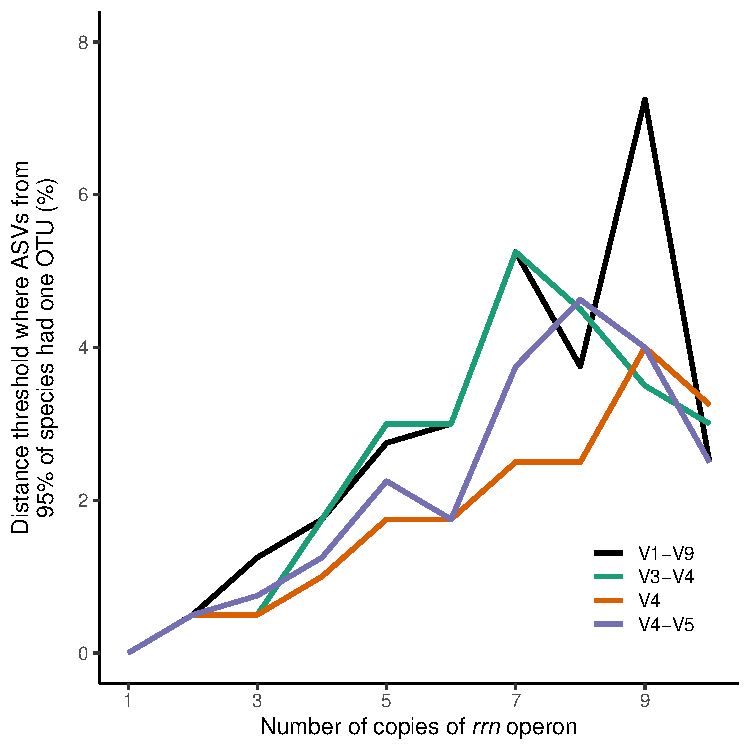
\includegraphics{../figures/copy_number_threshold_plot.pdf}

\textbf{Figure 1. The distance threshold required to prevent the
splitting of genomes into multiple OTUs increased as the number of
\emph{rrn} operons in the genome increased.} Each line represents the
median distance threshold for each region of the 16S rRNA gene that is
required for 95\% of the genomes with the indicated numbrer of
\emph{rrn} operons to cluster their ASVs to a single OTU. The median
distance threshold was calculated across 100 randomizations in which one
genome was sampled from each species. Only those number of \emph{rrn}
operons that were found in more than 100 species are included.

\newpage

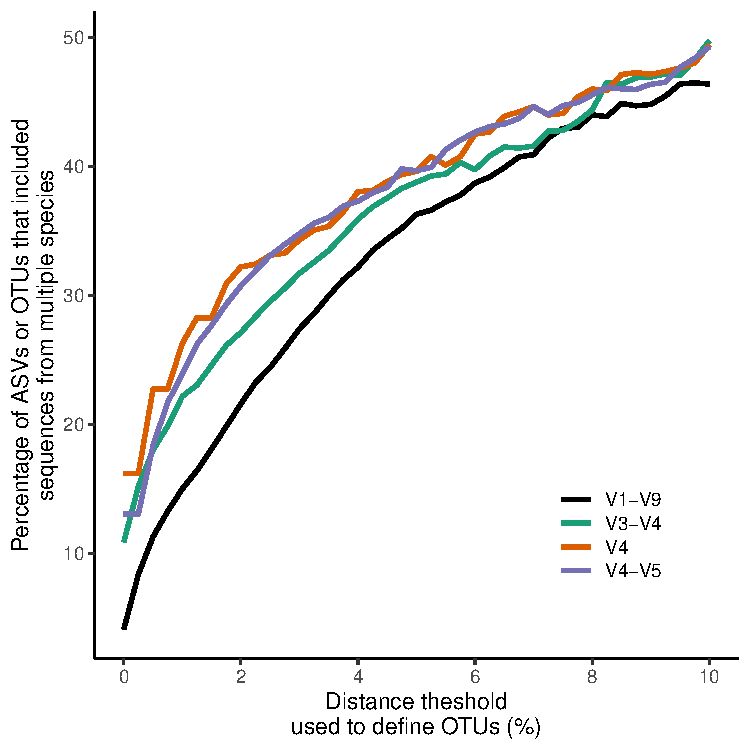
\includegraphics{../figures/lump_split.pdf}

\textbf{Figure 2. As the distance threshold used to define an OTU
increased, the fraction of genomes split into separate OTUs decreased
while the fraction of ASVs and OTUs representing multiple species
increased.} These data represent the median fractions for both
measurements across 100 randomizations. In each randomization, one
genome was sampled from each species.

\newpage

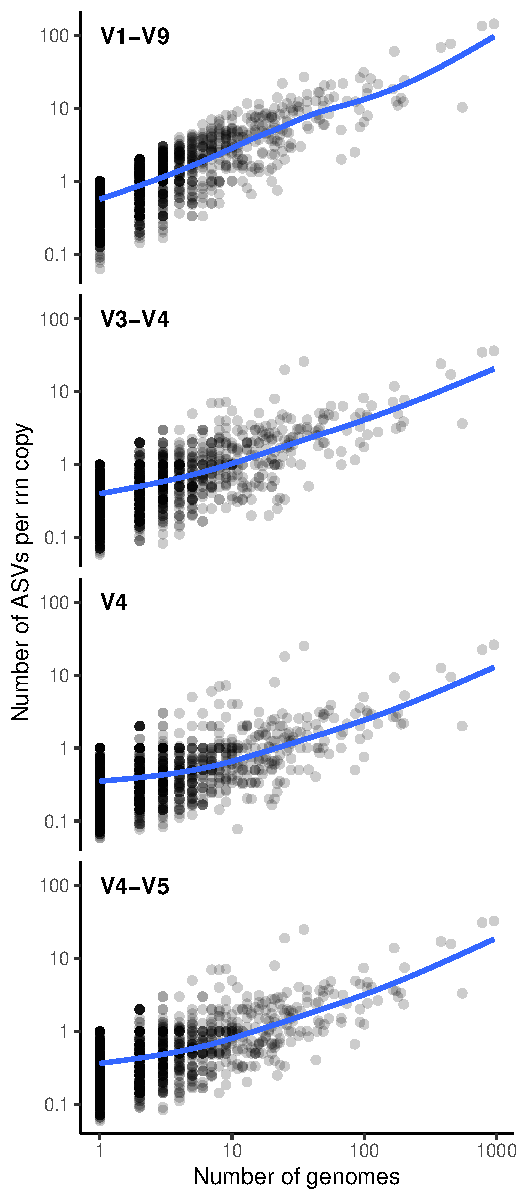
\includegraphics{../figures/esv_rate.pdf}

\textbf{Figure S1. The ratio of number of distinct ASVs per copy of the
\emph{rrn} operon increased for a species as the number of genomes in
the \emph{rrn}DB for that species increased.} Each point represents a
different species and was shaded to be 80\% transparent so that when
points overlap they become darker. The blue line represents a smoothed
fit through the data. Both axes use a logarithmic scale (base 10).

\end{document}
